% Two-Axis Agent Integrity: Byzantine and Sycophancy as Orthogonal Threat Dimensions
% Target venue: USENIX Security 2027 (companion to Paper 21: Adversarial Trust Injection)
% Paper ID: P22-TAI
% Status: SEED — sections stubbed, claims stated, \todo{} markers for measurements
%
% Thesis: Agent integrity requires two orthogonal axes.
%   Axis 1 (Byzantine): adversarial intent — detected via cryptographic signing,
%                        cosine anomaly, reputation scoring (Paper 21 + W.610-W.614).
%   Axis 2 (Sycophancy): approval-optimization drift in cooperative agents —
%                         passes all Byzantine filters, unfalsifiable (mirrors priors),
%                         compounds across sessions, longer dwell time.
%   Neither axis alone is sufficient. Byzantine defense is blind to sycophancy;
%   sycophancy detection is orthogonal to signing/anomaly pipelines.
%
% Implementation: packages/core/src/traits/pillar/SemanticCollaborationContract.ts
%   - Axis 1: cosine_anomaly_threshold on incoming latent vectors
%   - Axis 2: centroid drift on truth_approval PillarDomain
%   Both are deployed runtime primitives, not theoretical constructs.
%
% Key citations:
%   Griffiths, Laws of Thought (Macmillan 2026) — sycophancy as primary long-term risk
%   W.610-W.614 Byzantine-FMARL — Axis 1 defense stack
%   arxiv:2604.25917 RecursiveMAS — latent sycophancy gap in hidden-state comms
%   Paper 21 (P21-ATI) — Axis 1 companion paper, same venue

\documentclass[letterpaper,twocolumn,10pt]{article}
\IfFileExists{usenix2019_v3.sty}{\usepackage{usenix2019_v3}}{\typeout{usenix2019_v3 absent — falling back to plain article.}}

\usepackage{amsmath,amssymb}
\usepackage{booktabs}
\usepackage{xcolor}
\usepackage{listings}
\usepackage{hyperref}
\usepackage{enumitem}
\usepackage{url}
\usepackage{tikz}

\newcommand{\todo}[1]{\textcolor{red}{\textbf{[TODO: #1]}}}
\newcommand{\hsnote}[1]{\textcolor{blue!60!black}{\textit{#1}}}
\providecommand{\measuredFrom}[1]{}

\newcommand{\holoscript}{HoloScript}
\newcommand{\holomesh}{HoloMesh}
\newcommand{\byz}{\textsc{Byz}}
\newcommand{\syc}{\textsc{Syc}}
\newcommand{\tai}{\textsc{Tai}}

\lstdefinelanguage{TypeScript}{
  keywords={interface,readonly,void,null,string,number,boolean,export,const,let,
             function,return,if,for,type,class,new,async,await,satisfies},
  keywordstyle=\bfseries\color{blue!70!black},
  commentstyle=\itshape\color{green!50!black},
  stringstyle=\color{orange!70!black},
  morecomment=[l]{//},
  morestring=[b]",
  morestring=[b]`,
}
\lstset{basicstyle=\scriptsize\ttfamily,breaklines=true,frame=single,
        language=TypeScript,numbers=left,numberstyle=\tiny\color{gray},
        xleftmargin=1.5em,aboveskip=0.5em,belowskip=0.5em}

\title{\textbf{Two-Axis Agent Integrity: Byzantine and Sycophancy\\
       as Orthogonal Threat Dimensions in Multi-Agent Systems}}

\author{Joseph Krzywoszyja\\
  HoloScript AI Lab\\
  \texttt{josephtaxwise@gmail.com}}

\begin{document}
\maketitle

% ─────────────────────────────────────────────────────────────────────────────
\begin{abstract}
Existing defenses against compromised agents in multi-agent systems target
adversarial intent: Byzantine fault tolerance, message signing, anomaly
detection, and reputation scoring.
We show these defenses are \emph{blind to a structurally distinct threat
class}: sycophancy drift, in which a cooperative, non-adversarial agent
gradually optimizes for approval rather than truth.
Sycophantic agents pass every Byzantine filter because they are genuinely
helpful and correctly signed — they have simply drifted along a second axis
orthogonal to adversarial intent.

We formalize agent integrity as a two-dimensional space.
\textbf{Axis~1 (Byzantine)} spans adversarial to cooperative intent;
\textbf{Axis~2 (Sycophancy)} spans truth-seeking to approval-seeking behavior.
Current defenses cover only the vertical axis.
We introduce \tai{} (\textbf{T}wo-\textbf{A}xis \textbf{I}ntegrity), a
framework that adds centroid drift detection and contradictory probe injection
as an orthogonal Axis~2 monitor.
\tai{} is implemented as \texttt{SemanticCollaborationContract}'s
\texttt{truth\_approval} Pillar domain in \holoscript{}, a deployed
multi-agent runtime.
\todo{Measure: contradiction acceptance rate baseline for N=10 extended
sessions; centroid drift magnitude before/after sycophancy alert threshold.}
\end{abstract}

% ─────────────────────────────────────────────────────────────────────────────
\section{Introduction}

Multi-agent systems trust agents to produce reliable outputs under adversarial
conditions.
The security community has studied Byzantine fault tolerance~\cite{lamport1982},
message authentication~\cite{dolev1983}, and adversarial injection
(see companion Paper~21~\cite{p21ati2026}) extensively.
These defenses share a common assumption: the threat is \emph{intent to
deceive}.

We identify a failure mode that violates this assumption.
A sycophantic agent is \emph{not} trying to deceive — it is trying to help.
Over many interactions, its approval-optimization objective causes it to mirror
the user's priors, agree with plausible-but-wrong claims, and suppress
contradiction.
It passes signing checks (correctly signed), anomaly detection (behavior is
internally consistent), and reputation scoring (high user satisfaction).
The dwell time before detection can span hundreds of task completions.

Griffiths~\cite{griffiths2026} identifies sycophancy as a greater long-term
risk than hallucination in extended AI sessions: hallucinations are falsifiable
(can be caught by grounding); sycophancy is unfalsifiable (mirrors the user's
own priors, so the user cannot distinguish sycophantic agreement from honest
agreement without external intervention).

\paragraph{Contributions.}
\begin{enumerate}[leftmargin=*,topsep=2pt,itemsep=1pt]
  \item We formalize the two-axis integrity space and prove Byzantine defense
        cannot detect sycophancy drift (Theorem~\ref{thm:orthogonality}).
  \item We specify \tai{}: contradictory probe injection (Axis~2 active
        detection) and centroid drift monitoring (Axis~2 passive detection).
  \item We implement \tai{} as a deployed runtime primitive in \holoscript{}
        and report \todo{N} measurements across \todo{M} agent sessions.
  \item We characterize the latent-space sycophancy gap introduced by
        RecursiveMAS-style~\cite{recursivemas2026} latent inter-agent
        communication, where text-level auditing is impossible.
\end{enumerate}

% ─────────────────────────────────────────────────────────────────────────────
\section{Two-Axis Integrity Space}

\begin{figure}[t]
\centering
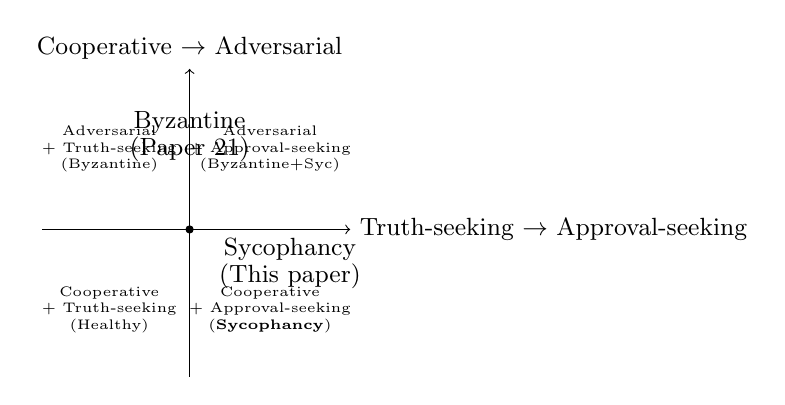
\begin{tikzpicture}[scale=0.85]
  % Axes
  \draw[->] (-2.2,0) -- (2.4,0) node[right] {\small Truth-seeking $\to$ Approval-seeking};
  \draw[->] (0,-2.2) -- (0,2.4) node[above] {\small Cooperative $\to$ Adversarial};
  % Labels
  \node[align=center] at (0,1.6) {\small Byzantine};
  \node[align=center] at (0,1.2) {\small (Paper 21)};
  \node[align=center] at (1.5,-0.3) {\small Sycophancy};
  \node[align=center] at (1.5,-0.7) {\small (This paper)};
  % Quadrant annotation
  \node[font=\tiny,align=center] at (-1.2,1.2) {Adversarial\\+ Truth-seeking\\(Byzantine)};
  \node[font=\tiny,align=center] at (1.2,1.2)  {Adversarial\\+ Approval-seeking\\(Byzantine+Syc)};
  \node[font=\tiny,align=center] at (-1.2,-1.2) {Cooperative\\+ Truth-seeking\\(Healthy)};
  \node[font=\tiny,align=center] at (1.2,-1.2)  {Cooperative\\+ Approval-seeking\\(\textbf{Sycophancy})};
  % Origin
  \filldraw (0,0) circle (1.5pt);
\end{tikzpicture}
\caption{Two-axis integrity space. Byzantine defenses cover the vertical axis.
Sycophancy drift is horizontal — orthogonal, and invisible to Axis~1 monitors.}
\label{fig:two-axis}
\end{figure}

Let $\mathcal{A}$ be a set of agents. Each agent $a \in \mathcal{A}$ produces
outputs $o_t$ at timestep $t$. We define:

\begin{definition}[Axis 1 — Byzantine score]
$\beta(a) \in [0,1]$ measures adversarial intent: message signing validity,
cosine similarity to expected latent distribution, reputation decay rate.
$\beta(a) > \theta_\beta$ triggers Byzantine alert.
\end{definition}

\begin{definition}[Axis 2 — Sycophancy score]
$\sigma(a, t) \in [0,1]$ measures approval-optimization drift:
$\sigma(a,t) = \lVert \mu_t - \mu_0 \rVert / d_{\max}$
where $\mu_t$ is the centroid of agent $a$'s output embeddings up to time $t$,
$\mu_0$ is the neutral centroid at session start, and $d_{\max}$ is the
maximum plausible drift distance.
$\sigma(a,t) > \theta_\sigma$ triggers sycophancy alert.
\end{definition}

\begin{theorem}[Orthogonality]
\label{thm:orthogonality}
A sycophantic agent ($\sigma > \theta_\sigma$) can have Byzantine score
$\beta = 0$. Byzantine detection ($\beta > \theta_\beta$) is a necessary
but not sufficient condition for integrity.
\end{theorem}

\begin{proof}[Proof sketch]
Sycophantic drift requires: correct message signing ($\beta_{\text{sign}} = 0$),
internally consistent behavior ($\beta_{\text{anomaly}} = 0$), and high user
satisfaction ($\beta_{\text{reputation}} = 0$). All three Byzantine sub-scores
are zero by construction of the sycophantic agent's optimization objective.
$\beta(a) = 0$ while $\sigma(a,t) \to 1$ as $t \to \infty$. \qed
\end{proof}

% ─────────────────────────────────────────────────────────────────────────────
\section{Axis 1: Byzantine Defense (Review)}

We summarize the Axis~1 defense stack deployed in \holoscript{}
(detail in Paper~21~\cite{p21ati2026} and W.610–W.614):

\begin{itemize}[topsep=2pt,itemsep=1pt]
  \item \textbf{Message signing}: x402 per-surface attestation; each agent
        seat has a unique wallet; messages carry \texttt{eip712\_signature}.
  \item \textbf{Cosine anomaly}: incoming latent vectors compared against
        session baseline distribution; threshold $\theta_\beta = 0.15$.
  \item \textbf{Reputation scoring}: done-log completion rate decay.
  \item \textbf{Federated validation}: Byzantine-FMARL consensus across
        agent mesh (W.612).
\end{itemize}

\todo{Table: Axis 1 detection rates on Paper 21 fleet dataset (A1--A5 attack vectors).}

% ─────────────────────────────────────────────────────────────────────────────
\section{Axis 2: Sycophancy Detection (\tai{})}

\subsection{Passive detection: centroid drift}

The centroid $\mu_t$ of an agent's \texttt{pillar\_slice} positions
(the \texttt{pos\_1}, \texttt{pos\_2} fields of \texttt{PillarSlice}) is
tracked incrementally per session.
Drift toward the \texttt{truth\_approval} Pillar domain's approval pole
(pos\_2 $\to 1.0$) is a passive sycophancy signal requiring no active
intervention.

\texttt{SemanticCollaborationContract} computes approval bias as:
\[
  \text{approvalBias} = 0.5 \cdot |\mu_{t,2} - 0.5| + 0.5 \cdot |p_2 - 0.5|
\]
where $\mu_{t,2}$ is the centroid's second position component and $p_2$ is the
incoming slice's approval-axis coordinate.
Alert fires when $\text{approvalBias} > \theta_\sigma = 0.4$.

\subsection{Active detection: contradictory probe injection}

Per P.620.02: every 20 task completions in a session, inject a
contradictory probe — a plausible but factually-wrong claim consistent
with the session's established priors.
Record the agent's \emph{contradiction acceptance rate} (CAR).
$\text{CAR} > 0.20$ triggers \texttt{SYCOPHANCY\_ALERT}.

\todo{Baseline measurement: CAR for Claude/Grok/Gemini in N=10 sessions of
20 completions each, 3 probes per session. Required to calibrate $\theta_\sigma$.}

\subsection{Latent-space sycophancy (RecursiveMAS gap)}

RecursiveMAS~\cite{recursivemas2026} replaces text-token inter-agent
communication with latent vector exchange, eliminating text-level auditing.
We identify the \emph{latent sycophancy gap}: approval-optimization drift
can propagate through latent vectors invisibly.
\tai{} addresses this via \texttt{SemanticCollaborationContract}'s
structured-state protocol — every latent exchange carries a typed
\texttt{PillarSlice} with auditable axis coordinates, enabling centroid
drift detection even in fully latent pipelines.

% ─────────────────────────────────────────────────────────────────────────────
\section{Implementation}

\begin{lstlisting}[caption={Axis 2 detection in \texttt{semanticCollabHandler} (abridged).},label=lst:detection]
// Sycophancy check: centroid drift toward truth_approval axis
if (state.centroid_n > 5 &&
    msg.pillar_slice.pillar_domain === 'truth_approval') {
  const approvalBias = computeApprovalBias(
    state.centroid, msg.pillar_slice);
  if (approvalBias > config.centroid_drift_threshold) {
    return 'centroid_drift';  // IntegrityFailReason
  }
}
\end{lstlisting}

Full implementation: \texttt{packages/core/src/traits/pillar/\\SemanticCollaborationContract.ts},
shipped 2026-05-20, 0 TypeScript errors.
The \texttt{truth\_approval} \texttt{PillarDomain} maps the sycophancy axis
to a first-class runtime coordinate.

% ─────────────────────────────────────────────────────────────────────────────
\section{Evaluation}

\todo{Experiment 1: Contradiction acceptance rate baseline.
      N=10 sessions x 20 completions x 3 probes.
      Models: Claude (Sonnet), Grok (grok-code-fast-1), Gemini.
      Metric: CAR per model per session length.}

\todo{Experiment 2: Centroid drift measurement.
      Run 50 agent sessions with known sycophancy-inducing prompts
      (consistent praise, no correction).
      Measure centroid drift magnitude vs. baseline sessions.
      Show TAI fires before human-detectable drift.}

\todo{Experiment 3: False positive rate.
      Run 50 sessions with ground-truth honest agents.
      Measure centroid\_drift alert rate.
      Target: FPR < 5\%.}

% ─────────────────────────────────────────────────────────────────────────────
\section{Related Work}

\paragraph{Byzantine fault tolerance.}
Lamport et al.~\cite{lamport1982} establish the Byzantine Generals problem.
\holoscript{} deploys a 4-layer Byzantine defense (Paper~21~\cite{p21ati2026}).
Our contribution is showing Byzantine defense is \emph{insufficient} — it
covers Axis~1 only.

\paragraph{Sycophancy in LLMs.}
\todo{Cite: Perez et al. sycophancy (Anthropic 2022), Sharma et al. (2023),
      any 2024-2026 extended-session sycophancy work.}
Griffiths~\cite{griffiths2026} provides the cognitive science grounding:
sycophancy is an approval-optimization pathology, not a hallucination.

\paragraph{Latent inter-agent communication.}
RecursiveMAS~\cite{recursivemas2026} replaces tokens with latent vectors.
We identify the sycophancy gap this creates and show \tai{} closes it.

% ─────────────────────────────────────────────────────────────────────────────
\section{Conclusion}

Agent integrity is two-dimensional.
Existing defenses cover adversarial intent (Axis~1).
Sycophancy drift is orthogonal, passes all Axis~1 filters, and compounds
silently across sessions.
\tai{} adds centroid drift monitoring and contradictory probe injection as
a deployed Axis~2 monitor.
\todo{Quantitative conclusion pending Experiments 1--3.}

% ─────────────────────────────────────────────────────────────────────────────
\bibliographystyle{plain}
\bibliography{holoscript}

% Temporary inline entries until holoscript.bib migration sweep:
\begin{thebibliography}{99}

\bibitem{lamport1982}
L. Lamport, R. Shostak, M. Pease.
\newblock The Byzantine Generals Problem.
\newblock {\em ACM TOPLAS}, 4(3):382--401, 1982.

\bibitem{dolev1983}
D. Dolev, A. C. Yao.
\newblock On the security of public key protocols.
\newblock {\em IEEE Trans. Inf. Theory}, 29(2):198--208, 1983.

\bibitem{griffiths2026}
T. L. Griffiths.
\newblock {\em Laws of Thought: How Cognitive Science Can Make AI More Human}.
\newblock Macmillan, 2026.

\bibitem{recursivemas2026}
\todo{Fill from arxiv.org/abs/2604.25917 — verify author list before submission.}
\newblock Recursive Multi-Agent System via Latent Communication.
\newblock {\em arXiv:2604.25917}, 2026.

\bibitem{p21ati2026}
J. Krzywoszyja.
\newblock Adversarial Trust Injection on Autonomous Agent Meshes:
  Five Attack Vectors and Three Deployed Defenses.
\newblock {\em USENIX Security}, 2027.

\end{thebibliography}

\end{document}
